%%%%%%%%%%%%%%%%%%%%%%%%%%%%%%%%%%%%%%%%%%%%%%%%%%%%%%%%%%%%%%%%%%%%%%%%%%%%%%%%%%
\begin{frame}[fragile]\frametitle{}
\begin{center}
{\Large Clustering}
\end{center}
\end{frame}

%%%%%%%%%%%%%%%%%%%%%%%%%%%%%%%%%%%%%%%%%%%%%%%%%%%%%%%%%%
\begin{frame}[fragile]\frametitle{The Problem}
\begin{itemize}
\item Imagine a storekeeper who keeps a record of all his customers' purchase histories. 
\item This allows him to look up the type of products an individual buyer might be interested in. 
\item However, doing this for each individual is grossly inefficient. 
\item A better solution would be to categorize his customers into groups, with each group having similar preferences. 
\item This would allow him to reach out to more customers with each product recommendation.
\end{itemize}
\end{frame}

%%%%%%%%%%%%%%%%%%%%%%%%%%%%%%%%%%%%%%%%%%%%%%%%%%%%%%%%%%
\begin{frame}[fragile]\frametitle{The Questions}
The problem is, the storekeeper does not know:
\begin{itemize}
\item How his customers should be categorized?
\item How many of such categories exist?
\end{itemize}
\end{frame}

%%%%%%%%%%%%%%%%%%%%%%%%%%%%%%%%%%%%%%%%%%%%%%%%%%%%%%%%%%
\begin{frame}[fragile]\frametitle{Clustering}
So, how do I discover natural groupings or segments in my data?
\begin{itemize}
\item Often we are given a large mass of data with no training labels. 
\item So we have no prior idea what to look for.
\item We can get some insight to get started, looking for similar items or ''clusters''
\end{itemize}
\end{frame}


%%%%%%%%%%%%%%%%%%%%%%%%%%%%%%%%%%%%%%%%%%%%%%%%%%%%%%%%%%%
%\begin{frame}[fragile]\frametitle{Clustering}
%\begin{itemize}
%\item  Unsupervised learning, Unlabeled data
%\item  Split observations into groups
%\item  Distance between data points
%\end{itemize}
%\end{frame}

%%%%%%%%%%%%%%%%%%%%%%%%%%%%%%%%%%%%%%%%%%%%%%%%%%%%%%%%%%
\begin{frame}[fragile]\frametitle{Clustering}
\begin{itemize}
\item  Organizing data into classes such that there is
\begin{itemize}
\item  High intra-class similarity
\item  Low inter-class similarity 
\end{itemize}
%\item  Finding the class labels and the number of classes directly from the data (in contrast to classification).
\item  More informally, finding natural groupings among objects. 
\end{itemize}
\begin{center}
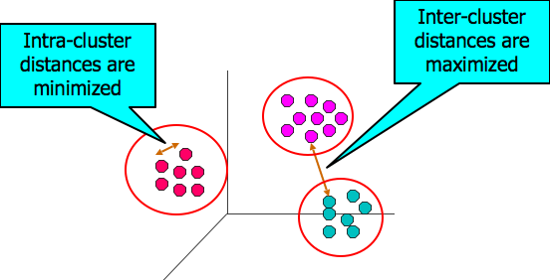
\includegraphics[width=0.5\linewidth,keepaspectratio]{clust}
\end{center}
\tiny{(Reference: Introduction to Data Mining - Tan, Steinbach, Kumar)}

\end{frame}

%%%%%%%%%%%%%%%%%%%%%%%%%%%%%%%%%%%%%%%%%%%%%%%%%%%%%%%%%%%%%%%%%%%%%%%%%%%%%%%%%%
\begin{frame}[fragile]\frametitle{}
\begin{center}
{\Large Types of Clustering}
\end{center}
\end{frame}


%%%%%%%%%%%%%%%%%%%%%%%%%%%%%%%%%%%%%%%%%%%%%%%%%%%%%%%%%%
\begin{frame}[fragile]\frametitle{Partition vs. Hierarchical}

\begin{itemize}
\item Partition Clustering: A division of data into non-overlapping clusters, such that each data object is in exactly one subset
\item Hierarchical Clustering: A set of nested clusters organized as a hierarchical tree 
\begin{itemize}
\item Each node (cluster) is union of its children (subclusters)
\item Root of tree: cluster containing all data objects
\item Leaves of tree: singleton clusters
\end{itemize}
\end{itemize}
\end{frame}

%%%%%%%%%%%%%%%%%%%%%%%%%%%%%%%%%%%%%%%%%%%%%%%%%%%%%%%%%%
\begin{frame}[fragile]\frametitle{Complete vs. Partial}

\begin{itemize}
\item Complete Clustering: Every object is assigned to a cluster
\item Partial Clustering: Not every object needs to be assigned
\begin{itemize}
\item Motivation: some objects in a dataset may not belong to well-defined groups
\item Noise, outliers, or simply ``uninteresting background'' data
\end{itemize}
\end{itemize}
\end{frame}


%%%%%%%%%%%%%%%%%%%%%%%%%%%%%%%%%%%%%%%%%%%%%%%%%%%%%%%%%%
\begin{frame}[fragile]\frametitle{Exclusive vs. Non-exclusive}

\begin{itemize}
\item Exclusive Clustering: Assignment is to one cluster
\item Non-Exclusive Clustering: Data objects may belong to multiple clusters
\begin{itemize}
\item Motivation: multi-class situations
\item Example: ``student employee''
\end{itemize}
\end{itemize}
Well-Separated Clusters: any point in a cluster is closer to every other point in the cluster than to any point not in the cluster
\begin{center}
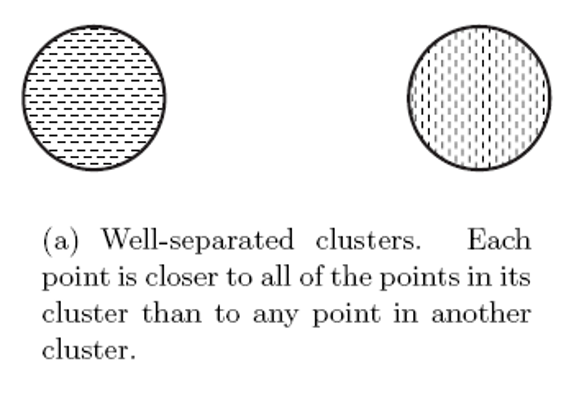
\includegraphics[width=0.5\linewidth,keepaspectratio]{wellclust}
\end{center}

\end{frame}

%%%%%%%%%%%%%%%%%%%%%%%%%%%%%%%%%%%%%%%%%%%%%%%%%%%%%%%%%%
\begin{frame}[fragile]\frametitle{Center-based Clusters}
\begin{itemize}
\item an object in a cluster is closer to the center of a cluster than to the center of any other cluster
\item Center of a cluster (``the most central point''): 
\begin{itemize}
\item Centroid: the mean of all the points in the cluster (usually for continuous attributes)
\item Medoid: the most ``representative'' point of a cluster (usually for categorical attributes)
\end{itemize}
\end{itemize}
\begin{center}
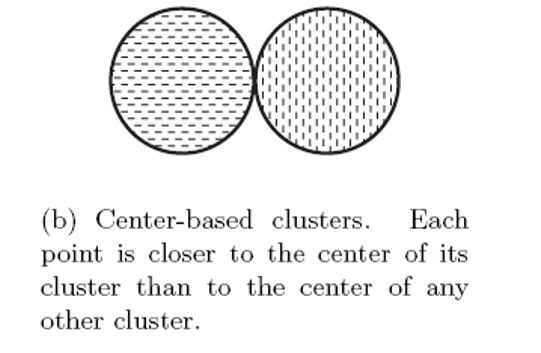
\includegraphics[width=0.5\linewidth,keepaspectratio]{centclust}
\end{center}
\end{frame}


%
%%%%%%%%%%%%%%%%%%%%%%%%%%%%%%%%%%%%%%%%%%%%%%%%%%%%%%%%%%%
%\begin{frame}[fragile]\frametitle{Hierarchical Clustering}
%\begin{itemize}
%\item Produces a set of nested clusters organized as a hierarchical tree
%\item Can be visualized as a dendrogram
%\item A tree like diagram that records the sequences of merges or splits
%\end{itemize}
%\begin{center}
%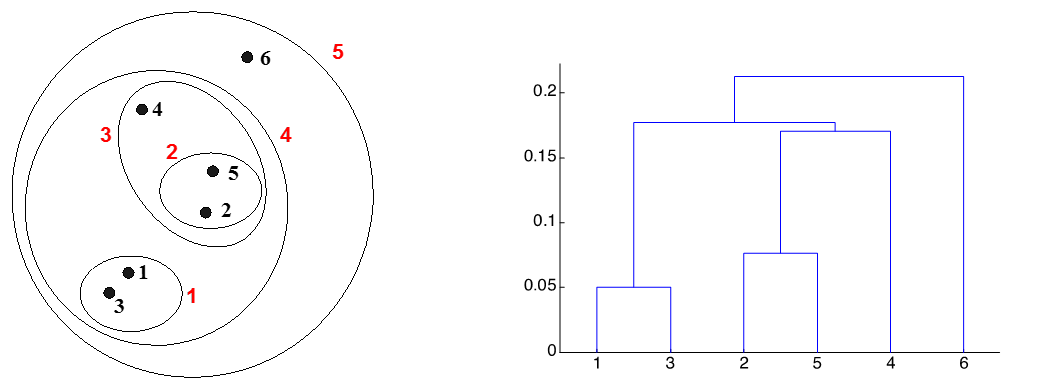
\includegraphics[width=\linewidth,keepaspectratio]{hierclust}
%\end{center}
%
%\end{frame}

%%%%%%%%%%%%%%%%%%%%%%%%%%%%%%%%%%%%%%%%%%%%%%%%%%%%%%%%%%%
%\begin{frame}[fragile]\frametitle{Hierarchical Clustering Approaches}
%\begin{itemize}
%\item Agglomerative: start with data points as individual clusters (bottom-up)
%\begin{itemize}
%\item at each step merge the closest pair of clusters
%\item Definition of ``cluster proximity'' needed.
%\end{itemize}
%\item Divisive: start with one all-inclusive cluster (top-down)
%\begin{itemize}
%\item at each step split a cluster until only singleton clusters remain
%\item Need to decide which cluster to split and how to do splitting
%\end{itemize}
%\end{itemize}
%\end{frame}

%%%%%%%%%%%%%%%%%%%%%%%%%%%%%%%%%%%%%%%%%%%%%%%%%%%%%%%%%%%
%\begin{frame}[fragile]\frametitle{Why Hierarchical Clustering?}
%\begin{itemize}
%\item Do not have to assume any particular number of clusters
%\begin{itemize}
%\item Any desired number of clusters can be obtained by 'cutting' the dendogram at the proper level
%\item Stopping the algorithm
%\end{itemize}
%\item They may correspond to meaningful taxonomies
%\begin{itemize}
%\item Example: biological sciences domain (e.g., animal kingdom, phylogeny reconstruction)
%\end{itemize}
%\end{itemize}
%\end{frame}
%
%%%%%%%%%%%%%%%%%%%%%%%%%%%%%%%%%%%%%%%%%%%%%%%%%%%%%%%%%%%
%\begin{frame}[fragile]\frametitle{Agglomerative Clustering Algorithm}
%\begin{itemize}
%\item Compute the proximity matrix
%\item Let each data point be a cluster
%\item Repeat
%	\begin{itemize}
%	\item Merge the two closest clusters
%	\item Update the proximity matrix
%	\end{itemize}
%\item Until only a single cluster remains
%\end{itemize}
%\end{frame}

%%%%%%%%%%%%%%%%%%%%%%%%%%%%%%%%%%%%%%%%%%%%%%%%%%%%%%%%%%%
%\begin{frame}[fragile]\frametitle{Hierarchical Clustering: Final Thoughts}
%\begin{itemize}
%\item Once a decision is made to combine two clusters, it cannot be undone
%\item More Advanced: Determining the Correct Number of Clusters
%\item Try different numbers of clusters
%\item Statistical measures used to help decide:: SSE
%
%\end{itemize}
%\end{frame}




%%%%%%%%%%%%%%%%%%%%%%%%%%%%%%%%%%%%%%%%%%%%%%%%%%%%%%%%%%%%%%%%%%%%%%%%%%%%%%%%%%
\begin{frame}[fragile]\frametitle{}
\begin{center}
{\Large Clustering Aspects}
\end{center}
\end{frame}

%%%%%%%%%%%%%%%%%%%%%%%%%%%%%%%%%%%%%%%%%%%%%%%%%%%%%%%%%%
\begin{frame}[fragile]\frametitle{Clustering}
Notion of a Cluster can be Ambiguous
\begin{center}
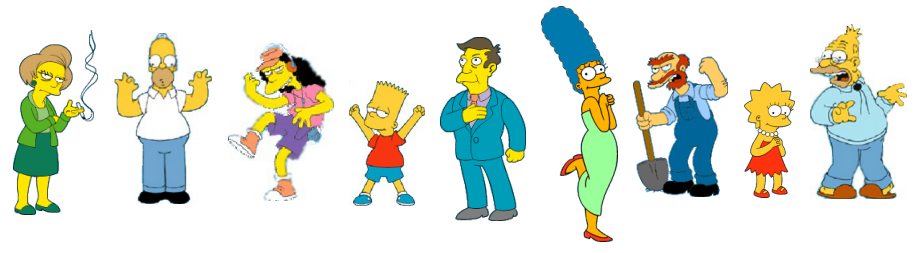
\includegraphics[width=0.8\linewidth,keepaspectratio]{kmns2}
\end{center}
\tiny{(Reference: K means Clustering Algorithm - 
Kasun Ranga Wijeweera)}
\end{frame}

%%%%%%%%%%%%%%%%%%%%%%%%%%%%%%%%%%%%%%%%%%%%%%%%%%%%%%%%%%
\begin{frame}[fragile]\frametitle{Clustering}
Notion of a Cluster can be Ambiguous
\begin{center}
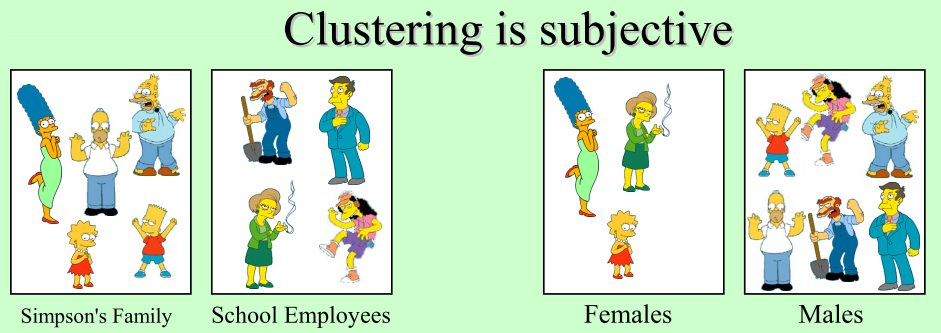
\includegraphics[width=0.8\linewidth,keepaspectratio]{kmns3}
\end{center}
\tiny{(Reference: K means Clustering Algorithm - 
Kasun Ranga Wijeweera)}
\end{frame}


%%%%%%%%%%%%%%%%%%%%%%%%%%%%%%%%%%%%%%%%%%%%%%%%%%%%%%%%%%
\begin{frame}[fragile]\frametitle{Clustering}
Notion of a Cluster can be Ambiguous
\begin{center}
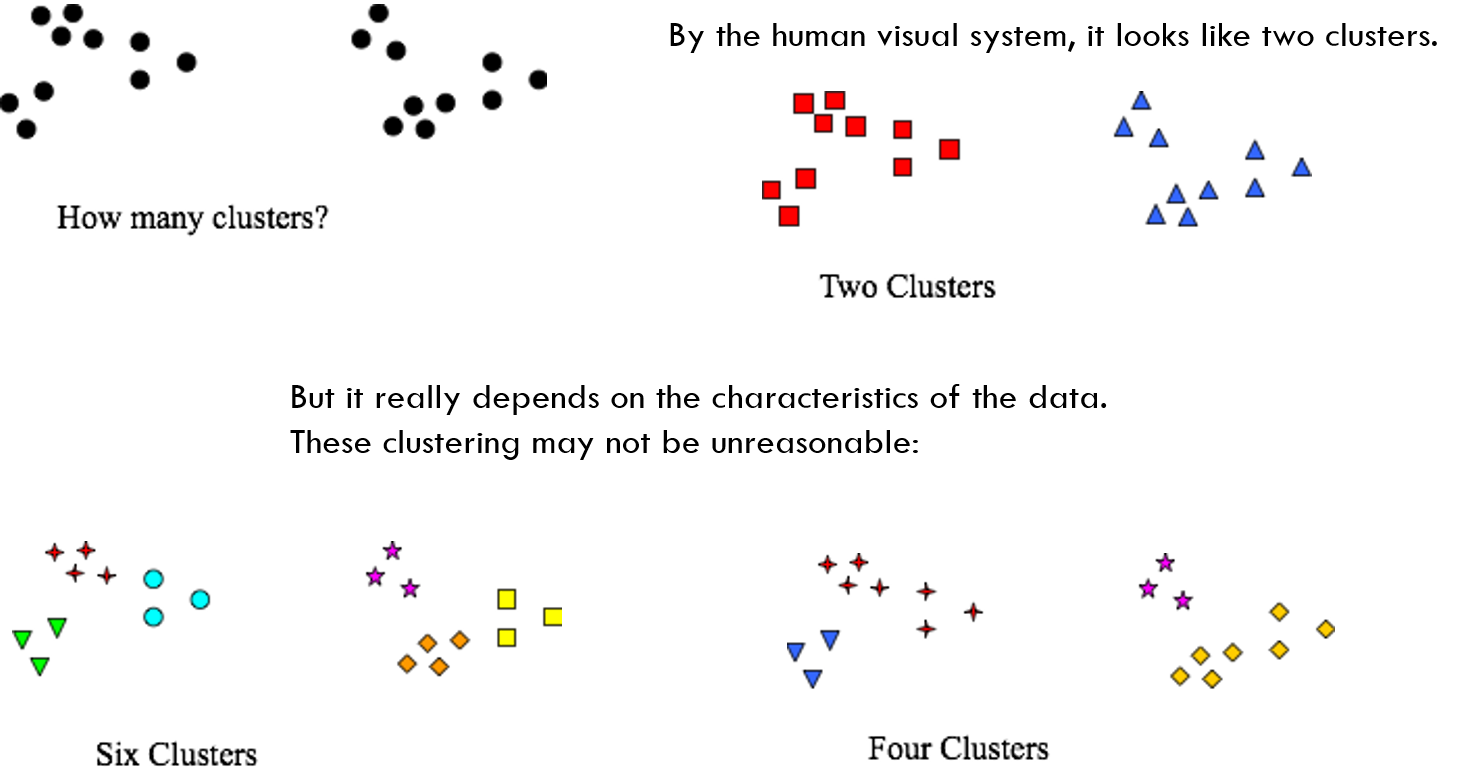
\includegraphics[width=0.8\linewidth,keepaspectratio]{clustamb}
\end{center}
\end{frame}

% %%%%%%%%%%%%%%%%%%%%%%%%%%%%%%%%%%%%%%%%%%%%%%%%%%%%%%%%%%%%%%%%%%%%%%%%%%%%%%%%%%
% \begin{frame}[fragile]\frametitle{}
% \begin{center}
% {\Large Clustering Algorithm}
% \end{center}
% \end{frame}


%%%%%%%%%%%%%%%%%%%%%%%%%%%%%%%%%%%%%%%%%%%%%%%%%%%%%%%%%%%%%%%%%%%%%%%%%%%%%%%%%%
\begin{frame}[fragile]\frametitle{}
\begin{center}
{\Large K-means}
\end{center}
\end{frame}


%%%%%%%%%%%%%%%%%%%%%%%%%%%%%%%%%%%%%%%%%%%%%%%%%%%%%%%%%%
\begin{frame}[fragile]\frametitle{Clustering}
\begin{itemize}
\item K-Means Clustering is one of the many techniques that constitute ''unsupervised learning''.
\item Creating a labeling of objects with cluster (class) labels
\item But, these labels are derived exclusively from the data.
\end{itemize}
\end{frame}

%%%%%%%%%%%%%%%%%%%%%%%%%%%%%%%%%%%%%%%%%%%%%%%%%%%%%%%%%%
\begin{frame}[fragile]\frametitle{K-Means Clustering}
\begin{itemize}
\item Formally: a method of vector quantization
\item Partition space into Voronoi cells
\item Separate samples into n groups of equal variance
\item Uses the Euclidean distance metric
\end{itemize}
\end{frame}

%%%%%%%%%%%%%%%%%%%%%%%%%%%%%%%%%%%%%%%%%%%%%%%%%%%%%%%%%%
\begin{frame}[fragile]\frametitle{K-Means Clustering}
\begin{center}
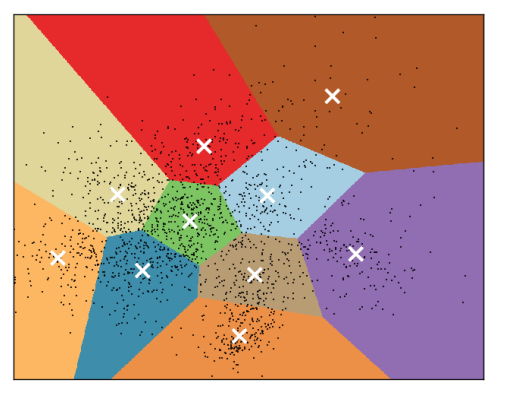
\includegraphics[width=0.6\linewidth,keepaspectratio]{kmns1}
\end{center}
\end{frame}

%%%%%%%%%%%%%%%%%%%%%%%%%%%%%%%%%%%%%%%%%%%%%%%%%%%%%%%%%%
\begin{frame}[fragile]\frametitle{Clustering by K-Means}
\begin{itemize}
%\item It is a type of unsupervised algorithm which  solves the clustering problem. 
\item It operates by computing the ''mean'' of some attributes. 
\item That ''mean'' then becomes the center of one cluster.
\item  Its procedure follows a simple and easy way to classify a given data set through a certain number of  clusters (assume k clusters). 
\item Data points inside a cluster are homogeneous and heterogeneous to peer groups.
\end{itemize}
\end{frame}
%%%%%%%%%%%%%%%%%%%%%%%%%%%%%%%%%%%%%%%%%%%%%%%%%%%%%%%%%%
\begin{frame}[fragile]\frametitle{How to cluster?}
\begin{itemize}
\item Clustering is different than prediction
\item Dividing data into groups (clusters) in some meaningful or useful way
\item Clustering should capture ``natural structure of the data''
\end{itemize}
\end{frame}

% %%%%%%%%%%%%%%%%%%%%%%%%%%%%%%%%%%%%%%%%%%%%%%%%%%%%%%%%%%
% \begin{frame}[fragile]\frametitle{How to cluster?}
% Finding groups of objects such that the objects within a group will be similar to one another and different from the objects in other groups

% \begin{center}
% 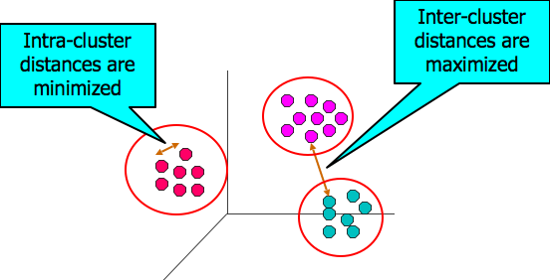
\includegraphics[width=\linewidth,keepaspectratio]{clust}
% \end{center}
% \end{frame}



%%%%%%%%%%%%%%%%%%%%%%%%%%%%%%%%%%%%%%%%%%%%%%%%%%%%%%%%%%
\begin{frame}[fragile]\frametitle{Clustering Algorithms}
\begin{itemize}
\item Clustering is different than prediction
\item K-nearest neighbors is very different from K-means, although both are somewhat based on `Similarity' or `Distance'
\item It is a classification (or regression) algorithm that in order to determine the classification of a point, 
\item Decides class of the test case based on the classes of the K nearest points. 
\item It is supervised because you are trying to classify a point based on the known classification of other points.)
\end{itemize}
\end{frame}



%%%%%%%%%%%%%%%%%%%%%%%%%%%%%%%%%%%%%%%%%%%%%%%%%%%%%%%%%%
\begin{frame}[fragile]\frametitle{How to cluster?}
\begin{itemize}
\item How to measure ``proximity''?
\item Proximity: similarity or dissimilarity between two objects
\item Similarity: numerical measure of the degree to which two objects are alike

\end{itemize}
%\begin{center}
%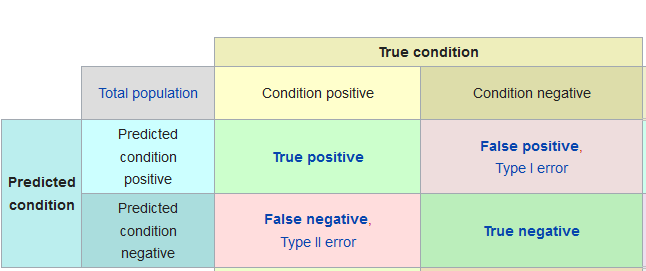
\includegraphics[width=\linewidth,keepaspectratio]{confmat}
%\end{center}

\end{frame}


%%%%%%%%%%%%%%%%%%%%%%%%%%%%%%%%%%%%%%%%%%%%%%%%%%%%%%%%%%%%%%%%%%%%%%%%%%%%%%%%%%
\begin{frame}[fragile]\frametitle{}
\begin{center}
{\Large Proximity - Distance Measures}
\end{center}
\end{frame}

%%%%%%%%%%%%%%%%%%%%%%%%%%%%%%%%%%%%%%%%%%%%%%%%%%%%%%%%%%
\begin{frame}[fragile]\frametitle{Defining Distance Measure/MetricS}
Say, some black box calculations.
\begin{center}
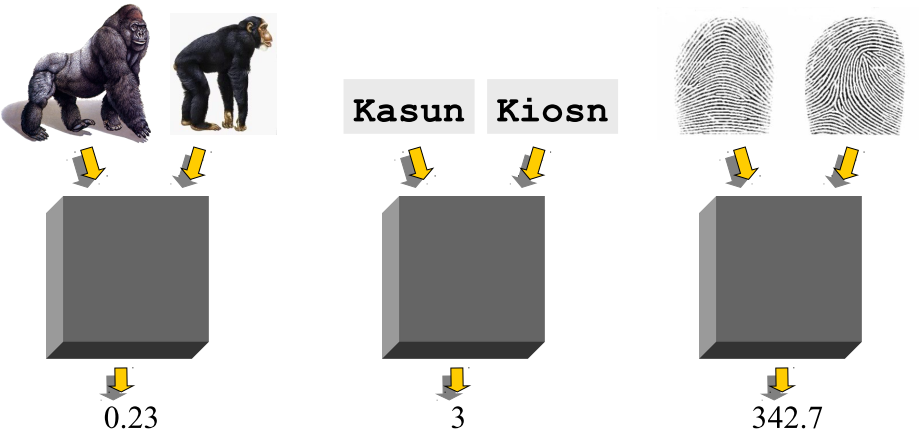
\includegraphics[width=\linewidth,keepaspectratio]{kmns4}
\end{center}
Some distance formulas.
\tiny{(Reference: K means Clustering Algorithm - 
Kasun Ranga Wijeweera)}
\end{frame}

%
%%%%%%%%%%%%%%%%%%%%%%%%%%%%%%%%%%%%%%%%%%%%%%%%%%%%%%%%%%%
%\begin{frame}[fragile]\frametitle{Distance Metric}
%\begin{itemize}
%\item Distance Metric: A function that returns the distance between two instances a and b.
%\item Must, mathematically have the criteria:
%	\begin{itemize}
%	\item Non-negativity $dist(a,b)\ge 0$
%	\item Identity $dist(a,b)= 0, a =b$
%	\item Symmetry $dist(a,b)= dist(b,a)$
%	\item Triangular Inequality:  $dist(a,c)\leq dist(a,b) \leq dist(b,c)$
%	\end{itemize}
%\end{itemize}
%\end{frame}

%%%%%%%%%%%%%%%%%%%%%%%%%%%%%%%%%%%%%%%%%%%%%%%%%%%%%%%%%%
\begin{frame}[fragile]\frametitle{Dissimilarities between Data Objects}
\begin{itemize}
\item A common measure for the proximity between two objects is the Euclidean Distance
\item Defined for one-dimension, two-dimensions, three-dimensions, any n-dimensional space
\item Generically: Minkowski Distance Metric
	\begin{itemize}
	\item $r=1$ : $L_1$ norm: Manhattan or Taxi cab distance
	\item $r=2$ : $L_2$ norm: Euclidean distance
	\end{itemize}
%
%\item So far, all attributes treated equally when computing proximity
%\item In some situations: some features are more important than others. Decision up to the analyst
\end{itemize}
\end{frame}

%%%%%%%%%%%%%%%%%%%%%%%%%%%%%%%%%%%%%%%%%%%%%%%%%%%%%%%%%%
\begin{frame}[fragile]\frametitle{Example}
\begin{center}
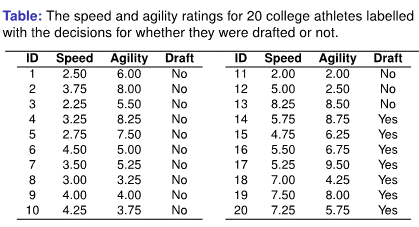
\includegraphics[width=0.8\linewidth,keepaspectratio]{distexam}
\end{center}
$d(id_{12},id_5) = \sqrt{(5.00 - 2.75)^2 + (2.50 - 7.50)^2} = \sqrt{30.0625} = 5.4829$
\end{frame}

%%%%%%%%%%%%%%%%%%%%%%%%%%%%%%%%%%%%%%%%%%%%%%%%%%%%%%%%%%
\begin{frame}[fragile]\frametitle{Distance Matrix}
\begin{itemize}
\item Once a distance metric is chosen, the proximity between all of the objects in the dataset can be computed
\item Can be represented in a distance matrix
\item Pairwise distances between points
\end{itemize}
\begin{center}
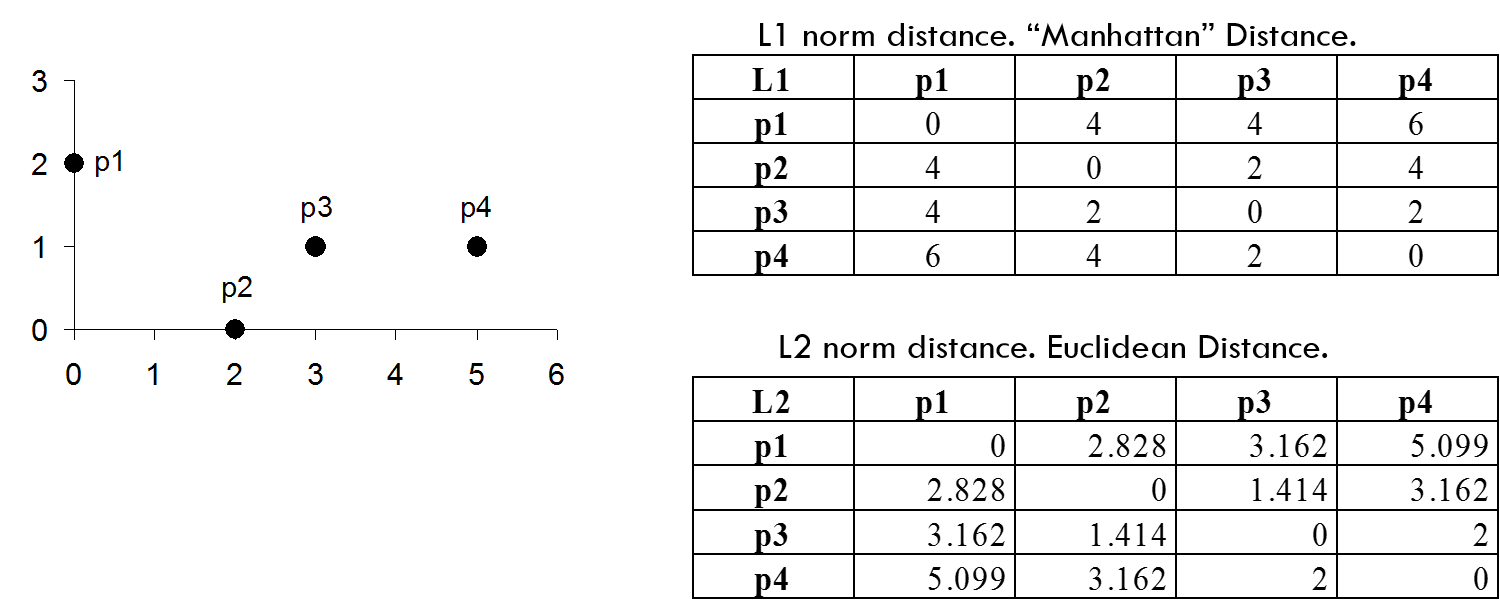
\includegraphics[width=0.8\linewidth,keepaspectratio]{pairdist}
\end{center}
\end{frame}

%%%%%%%%%%%%%%%%%%%%%%%%%%%%%%%%%%%%%%%%%%%%%%%%%%%%%%%%%%%%%%%%%%%%%%%%%%%%%%%%%%
\begin{frame}[fragile]\frametitle{}
\begin{center}
{\Large K-means Algorithm}
\end{center}
\end{frame}

%%%%%%%%%%%%%%%%%%%%%%%%%%%%%%%%%%%%%%%%%%%%%%%%%%%%%%%%%%
\begin{frame}[fragile]\frametitle{How  K-means forms cluster?}
Algorithm
\begin{itemize}
\item  Iterative refinement
\item  Three basic steps
\item  Step 1: Choose k
\item  Iterate over:
\begin{itemize}
\item  Step 2: Assignment
\item  Step 3: Update centroids
\end{itemize}
\item  Repeats until convergence has been reached
\end{itemize}
\end{frame}

% %%%%%%%%%%%%%%%%%%%%%%%%%%%%%%%%%%%%%%%%%%%%%%%%%%%%%%%%%%
% \begin{frame}[fragile]\frametitle{Algorithm: Mathematically}
% Consider a set of data points
% \begin{center}
% 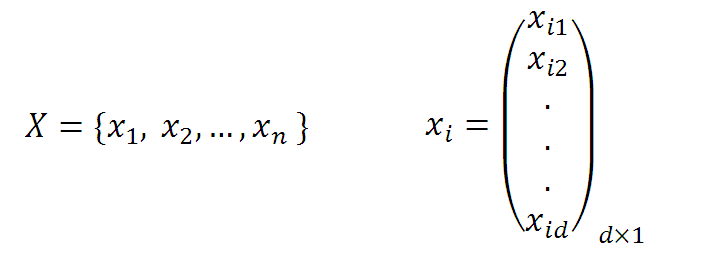
\includegraphics[width=0.8\linewidth,keepaspectratio]{kmns5}
% \end{center}
% and a set of clusters
% \begin{center}
% 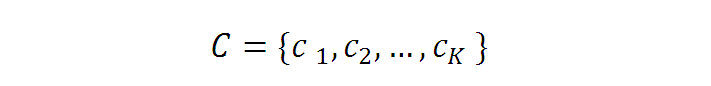
\includegraphics[width=0.8\linewidth,keepaspectratio]{kmns6}
% \end{center}
% \end{frame}

% %%%%%%%%%%%%%%%%%%%%%%%%%%%%%%%%%%%%%%%%%%%%%%%%%%%%%%%%%%
% \begin{frame}[fragile]\frametitle{Algorithm: The Goal}
% \begin{center}
% 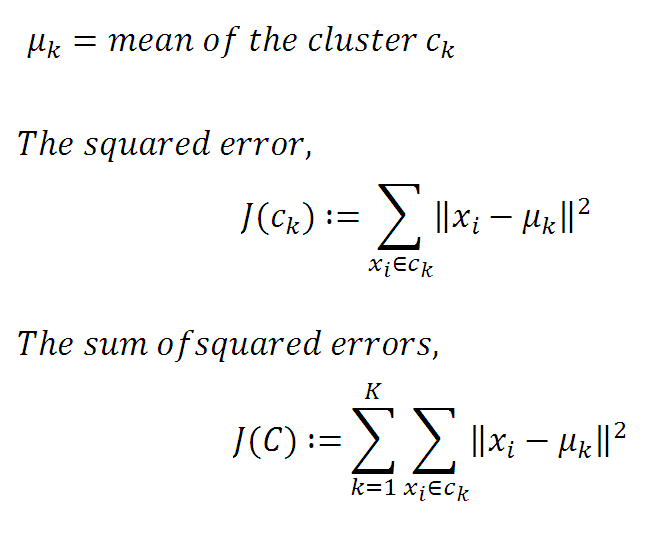
\includegraphics[width=0.7\linewidth,keepaspectratio]{kmns7}
% \end{center}
% \end{frame}

%%%%%%%%%%%%%%%%%%%%%%%%%%%%%%%%%%%%%%%%%%%%%%%%%%%%%%%%%%
\begin{frame}[fragile]\frametitle{How  K-means forms cluster?}
Algorithm
\begin{enumerate}
\item  K-means picks k points known as centroids.
\item  Each data point finds distances with each centroid and goes to the one who is closest.
\item In the next iteration, it computes a new centroid of each cluster based on the latest cluster members.
\item As we have new centroids, repeat step 2 and 3. 
\item Repeat this process until convergence occurs i.e. centroids do not change.
\end{enumerate}
\end{frame}

%%%%%%%%%%%%%%%%%%%%%%%%%%%%%%%%%%%%%%%%%%%%%%%%%%%%%%%%%%%
%\begin{frame}[fragile]\frametitle{Algorithm: Steps}
%\begin{center}
%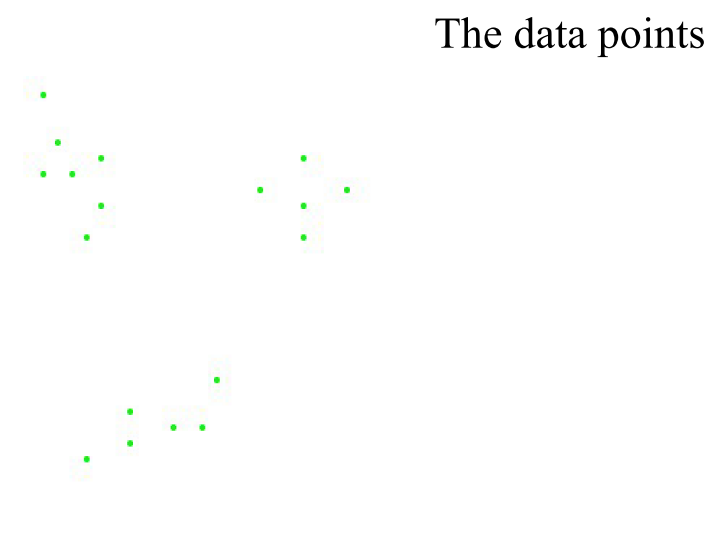
\includegraphics[width=\linewidth,keepaspectratio]{kmns8}
%\end{center}
%\end{frame}
%
%%%%%%%%%%%%%%%%%%%%%%%%%%%%%%%%%%%%%%%%%%%%%%%%%%%%%%%%%%%
%\begin{frame}[fragile]\frametitle{Algorithm: Steps}
%\begin{center}
%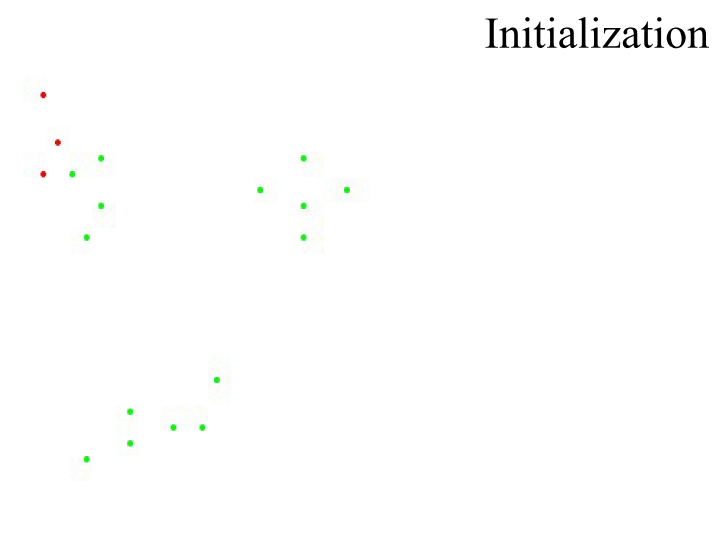
\includegraphics[width=\linewidth,keepaspectratio]{kmns9}
%\end{center}
%\end{frame}
%
%%%%%%%%%%%%%%%%%%%%%%%%%%%%%%%%%%%%%%%%%%%%%%%%%%%%%%%%%%%
%\begin{frame}[fragile]\frametitle{Algorithm: Steps}
%\begin{center}
%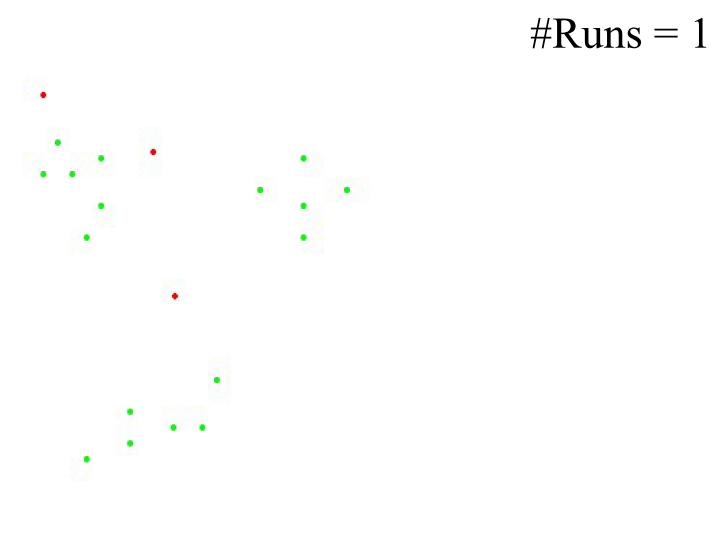
\includegraphics[width=\linewidth,keepaspectratio]{kmns10}
%\end{center}
%\end{frame}
%
%%%%%%%%%%%%%%%%%%%%%%%%%%%%%%%%%%%%%%%%%%%%%%%%%%%%%%%%%%%
%\begin{frame}[fragile]\frametitle{Algorithm: Steps}
%\begin{center}
%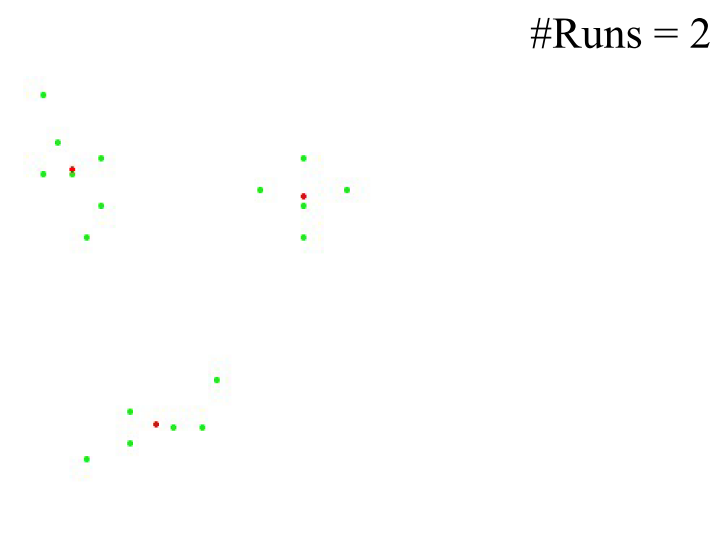
\includegraphics[width=\linewidth,keepaspectratio]{kmns11}
%\end{center}
%\end{frame}
%
%%%%%%%%%%%%%%%%%%%%%%%%%%%%%%%%%%%%%%%%%%%%%%%%%%%%%%%%%%%
%\begin{frame}[fragile]\frametitle{Algorithm: Steps}
%\begin{center}
%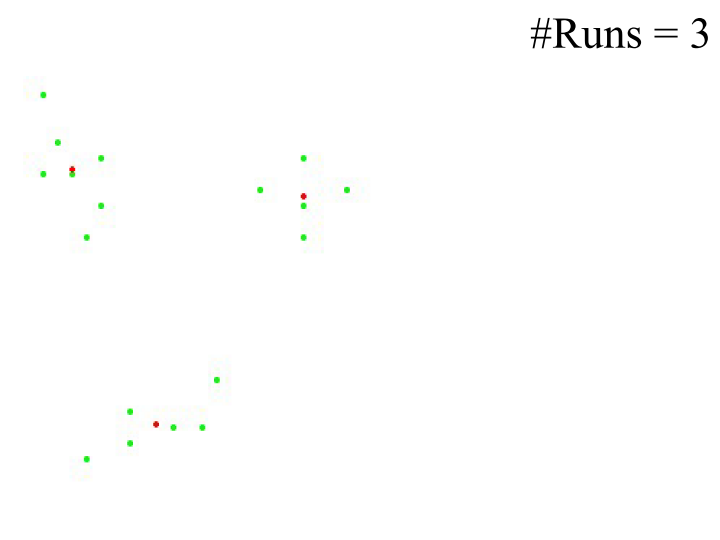
\includegraphics[width=\linewidth,keepaspectratio]{kmns12}
%\end{center}
%\end{frame}



%%%%%%%%%%%%%%%%%%%%%%%%%%%%%%%%%%%%%%%%%%%%%%%%%%%%%%%%%%
\begin{frame}[fragile]\frametitle{Algorithm: Steps}
\begin{itemize}
\item  Data points are K=2 given. 
\item So random two points are chosen as centroids
\end{itemize}

\begin{center}
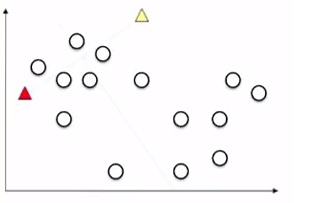
\includegraphics[width=0.5\linewidth,keepaspectratio]{kmns15}
\end{center}
\end{frame}

%%%%%%%%%%%%%%%%%%%%%%%%%%%%%%%%%%%%%%%%%%%%%%%%%%%%%%%%%%
\begin{frame}[fragile]\frametitle{Algorithm: Steps}
\begin{itemize}
\item  Each data point is assigned to closest centroid
\item Closeness is based on Distance
\end{itemize}
\begin{center}
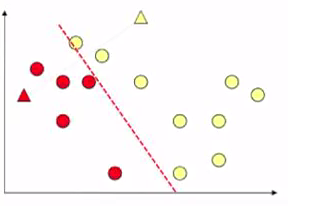
\includegraphics[width=0.5\linewidth,keepaspectratio]{kmns16}
\end{center}
\end{frame}

%%%%%%%%%%%%%%%%%%%%%%%%%%%%%%%%%%%%%%%%%%%%%%%%%%%%%%%%%%
\begin{frame}[fragile]\frametitle{Algorithm: Steps}
\begin{itemize}
\item Calculate new centroids of respective groups
\item By averaging NUMERIC variables only.
\end{itemize}
\begin{center}
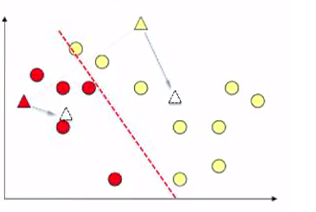
\includegraphics[width=0.5\linewidth,keepaspectratio]{kmns17}
\end{center}
\end{frame}


%%%%%%%%%%%%%%%%%%%%%%%%%%%%%%%%%%%%%%%%%%%%%%%%%%%%%%%%%%
\begin{frame}[fragile]\frametitle{Algorithm: Steps}
\begin{itemize}
\item Repeat.
\item Memberships may change now.
\item Update till centroids don't move appreciably.
\item Clustering is DONE.
\end{itemize}
\begin{center}
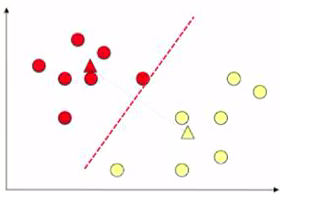
\includegraphics[width=0.5\linewidth,keepaspectratio]{kmns18}
\end{center}
\end{frame}


%%%%%%%%%%%%%%%%%%%%%%%%%%%%%%%%%%%%%%%%%%%%%%%%%%%%%%%%%%%%%%%%%%%%%%%%%%%%%%%%%%
\begin{frame}[fragile]\frametitle{}
\begin{center}
{\Large K-Means Implementation}
\end{center}
\end{frame}


%%%%%%%%%%%%%%%%%%%%%%%%%%%%%%%%%%%%%%%%%%%%%%%%%%%%%%%%%%%
\begin{frame}[fragile]\frametitle{K-means Algorithm : From Scratch}
Load data
\begin{lstlisting}
data = loadmat('data/ex7data2.mat')
X = data['X']
\end{lstlisting}
\end{frame}

%%%%%%%%%%%%%%%%%%%%%%%%%%%%%%%%%%%%%%%%%%%%%%%%%%%%%%%%%%%
\begin{frame}[fragile]\frametitle{K-means Algorithm : From Scratch}
A function that finds the closest centroid for each instance in the data:
\begin{lstlisting}
def find_closest_centroids(X, centroids):
    m = X.shape[0]
    k = centroids.shape[0]
    idx = np.zeros(m)
    
    for i in range(m):
        min_dist = 1000000
        for j in range(k):
            dist = np.sum((X[i,:] - centroids[j,:]) ** 2)
            if dist < min_dist:
                min_dist = dist
                idx[i] = j
    
    return idx
\end{lstlisting}
\end{frame}

%%%%%%%%%%%%%%%%%%%%%%%%%%%%%%%%%%%%%%%%%%%%%%%%%%%%%%%%%%%
\begin{frame}[fragile]\frametitle{K-means Algorithm : From Scratch}
Test
\begin{lstlisting}
initial_centroids = np.array([[3, 3], [6, 2], [8, 5]])

idx = find_closest_centroids(X, initial_centroids)

idx[0:3]
array([ 0.,  2.,  1.])
\end{lstlisting}
Cluster Ids
\end{frame}


%%%%%%%%%%%%%%%%%%%%%%%%%%%%%%%%%%%%%%%%%%%%%%%%%%%%%%%%%%%
\begin{frame}[fragile]\frametitle{K-means Algorithm : From Scratch}
A function to compute the centroid of a cluster:
\begin{lstlisting}
def compute_centroids(X, idx, k):
    m, n = X.shape
    centroids = np.zeros((k, n))
    
    for i in range(k):
        indices = np.where(idx == i)
        centroids[i,:] = (np.sum(X[indices,:], axis=1) /
        					len(indices[0])).ravel() 
    return centroids
    
compute_centroids(X, idx, 3)
array([[ 2.42830111,  3.15792418],
       [ 5.81350331,  2.63365645],
       [ 7.11938687,  3.6166844 ]])
\end{lstlisting}
\end{frame}

%%%%%%%%%%%%%%%%%%%%%%%%%%%%%%%%%%%%%%%%%%%%%%%%%%%%%%%%%%%
\begin{frame}[fragile]\frametitle{K-means Algorithm : From Scratch}
We can init centroids using some random sample of data-points as well
\begin{lstlisting}
def init_centroids(X, k):
    m, n = X.shape
    centroids = np.zeros((k, n))
    idx = np.random.randint(0, m, k)
    for i in range(k):
        centroids[i,:] = X[idx[i],:]
    return centroids
    
init_centroids(X, 3)
array([[ 1.15354031,  4.67866717],
       [ 6.27376271,  2.24256036],
       [ 2.20960296,  4.91469264]])
\end{lstlisting}
\end{frame}



%%%%%%%%%%%%%%%%%%%%%%%%%%%%%%%%%%%%%%%%%%%%%%%%%%%%%%%%%%%
\begin{frame}[fragile]\frametitle{K-means Algorithm : From Scratch}
Core
\begin{lstlisting}
def run_k_means(X, initial_centroids, max_iters):
    m, n = X.shape
    k = initial_centroids.shape[0]
    idx = np.zeros(m)
    centroids = initial_centroids
    
    for i in range(max_iters):
        idx = find_closest_centroids(X, centroids)
        centroids = compute_centroids(X, idx, k)
    
    return idx, centroids
\end{lstlisting}
\end{frame}

%%%%%%%%%%%%%%%%%%%%%%%%%%%%%%%%%%%%%%%%%%%%%%%%%%%%%%%%%%%
\begin{frame}[fragile]\frametitle{K-means Algorithm : From Scratch}
Run
\begin{lstlisting}
idx, centroids = run_k_means(X, initial_centroids, 10)

cluster1 = X[np.where(idx == 0)[0],:]
cluster2 = X[np.where(idx == 1)[0],:]
cluster3 = X[np.where(idx == 2)[0],:]
\end{lstlisting}
\end{frame}

%%%%%%%%%%%%%%%%%%%%%%%%%%%%%%%%%%%%%%%%%%%%%%%%%%%%%%%%%%%
\begin{frame}[fragile]\frametitle{K-means Algorithm : From Scratch}
Plot
\begin{lstlisting}
fig, ax = plt.subplots(figsize=(12,8))
ax.scatter(cluster1[:,0], cluster1[:,1], s=30, color='r', label='Cluster 1')
ax.scatter(cluster2[:,0], cluster2[:,1], s=30, color='g', label='Cluster 2')
ax.scatter(cluster3[:,0], cluster3[:,1], s=30, color='b', label='Cluster 3')
ax.legend()
\end{lstlisting}
\begin{center}
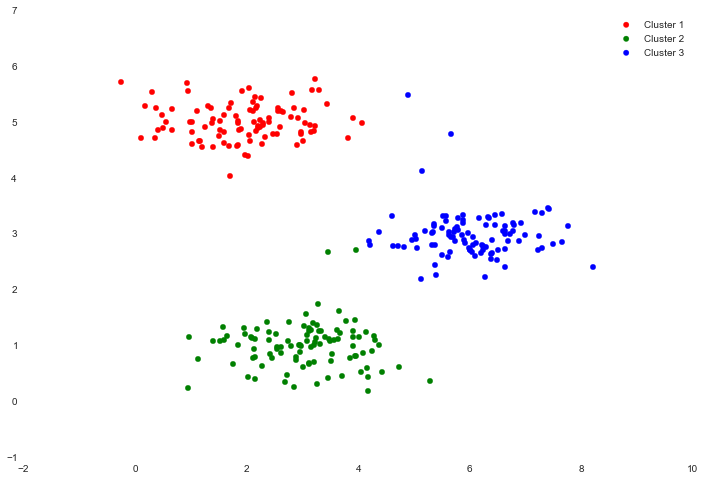
\includegraphics[width=0.5\linewidth,keepaspectratio]{kmns13}
\end{center}
\end{frame}



%%%%%%%%%%%%%%%%%%%%%%%%%%%%%%%%%%%%%%%%%%%%%%%%%%%%%%%%%%%%%%%%%%%%%%%%%%%%%%%%%%
\begin{frame}[fragile]\frametitle{}
\begin{center}
{\Large Summary}
\end{center}
\end{frame}

%%%%%%%%%%%%%%%%%%%%%%%%%%%%%%%%%%%%%%%%%%%%%%%%%%%%%%%%%%
\begin{frame}[fragile]\frametitle{Algorithm: Summary}
\begin{center}
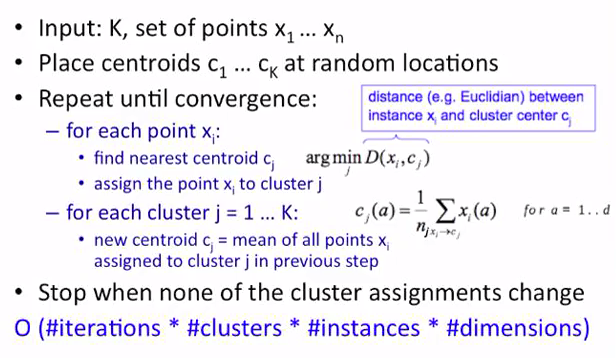
\includegraphics[width=0.8\linewidth,keepaspectratio]{kmns14}
\end{center}

(Note: Only numeric attributes can be averaged for centroid calculations)

\tiny{(Reference: K Means Clustering - Victor Lavrenko)}
\end{frame}


%%%%%%%%%%%%%%%%%%%%%%%%%%%%%%%%%%%%%%%%%%%%%%%%%%%%%%%%%%
\begin{frame}[fragile]\frametitle{K-means}
\begin{itemize}
\item  Advantages
\begin{itemize}
\item  Scales well
\item   Efficient
\end{itemize}
\item  Disadvantages
\begin{itemize}
\item Choosing the wrong k
\end{itemize}
\end{itemize}
\end{frame}

%%%%%%%%%%%%%%%%%%%%%%%%%%%%%%%%%%%%%%%%%%%%%%%%%%%%%%%%%%
\begin{frame}[fragile]\frametitle{K-means}
When to use?
\begin{itemize}
\item  Normally distributed data
\item  Large number of samples
\item  Not too many clusters
\item  Distance can be measured in a linear fashion
\end{itemize}
\end{frame}



%%%%%%%%%%%%%%%%%%%%%%%%%%%%%%%%%%%%%%%%%%%%%%%%%%%%%%%%%%
\begin{frame}[fragile]\frametitle{Applications}
\begin{itemize}
%\item Starting point for data summarization
%\item Understanding (human beings are good at dividing things into groups that share common characteristics)
\item Business
	\begin{itemize}
	\item Businesses collect large amounts of information on current and potential customers.
	\item Clustering to segment customers into a small number of groups, for additional analysis and marketing activities
	\end{itemize}
\item Clustering for Utility
	\begin{itemize}
	\item Efficiently Finding Nearest Neighbors
	\item Alternative to computing the pairwise distance between all points
	\end{itemize}
\end{itemize}
\end{frame}



